\documentclass{tikznotes}
%-----   封面信息   -----
\title{tikz笔记}
\author{樊超}
\date{\today}
\definecolor{mycolor}{rgb}{255,106,106}
\tcbset{
	colback=red!5!white,colframe=red!50,colbacktitle=red!75!black,fonttitle=\rmfamily\bfseries\large,coltitle=black,widget,
}
%-----  代码存放处  -----
%listing side text 左右


%\begin{tcblisting}{listing and text}  
%
%\end{tcblisting}
\begin{document}
\maketitle

\section{一维}

\subsection{点}

\begin{tcblisting}{listing outside text,righthand width=3cm}  


\begin{tikzpicture}
\fill (0,0) circle (2pt);
\end{tikzpicture}

\end{tcblisting}

\subsection{线}

\begin{tcblisting}{listing outside text,righthand width=3cm}  
你\tikz\draw(0pt,0pt)--(30pt,6pt);好
\end{tcblisting}

\begin{tcblisting}{listing side text,righthand width=3cm}  
你\tikz{\draw(0pt,0pt)--(30pt,6pt);}好
\end{tcblisting}

\begin{tcblisting}{listing side text,righthand width=3cm,title={线的粗细}}  

\begin{tikzpicture}
\draw[line width=3pt](0,0)--(3,0);
\draw[ultra thick](0,-.5)--(3,-.5);
\draw[very thick](0,-1)--(3,-1);
\draw[thick](0,-1.5)--(3,-1.5);
\draw[thin](0,-2)--(3,-2);
\draw[very thin](0,-2.5)--(3,-2.5);
\draw[ultra thin](0,-3)--(3,-3);
\end{tikzpicture}
\end{tcblisting}

\begin{tcblisting}{listing side text,righthand width=3cm,title={不同类型的线},widget}  
\begin{tikzpicture}
\draw[dash pattern=on 20pt off 10pt](0,-.5)--(3,-.5);
\draw[dash dot dot](0,-1.5)--(3,-1.5);
\draw[dash dot](0,-2)--(3,-2);
\draw[densely dotted](0,-2.5)--(3,-2.5);
\draw[dotted](0,-3)--(3,-3);
\draw[dotted](0,-3.5)--(3,-3.5);
\draw[dashed](0,-4)--(3,-4);
\draw[dashed](0,-4.5--(3,-4.5);
\end{tikzpicture}
\end{tcblisting}


\begin{tcblisting}{listing and text,title={不同类型的线},widget}  
\begin{tikzpicture}
\draw[dash pattern=on 20pt off 10pt,dash phase=10pt](0,0)--(3,0);
\draw[dash pattern=on 2pt off 3pt on 3pt off 2pt](0,-.5)--(3,-.5);
\end{tikzpicture}
\end{tcblisting}

\subsection{箭头}
\myverb{\usetikzlibrary {arrows.meta}}

\begin{tcblisting}{listing side text,righthand width=3cm,title={普通}}  
\begin{tikzpicture} 
\draw[->] (0,3) -- (3,3); 
\draw[->>] (0,2) -- (3,2); 
\draw[->|] (0,1) -- (3,1); 
\draw[-to] (0,0) -- (3,0); 
\draw[-latex] (0,-1) -- (3,-1); 
\draw[latex-latex] (0,-2) -- (3,-2); 
\draw[-stealth] (0,-3) -- (3,-3);
\draw[->] (2,-4).. controls +(left:5mm) and +(up:5mm)..(1,-5);
\end{tikzpicture}
\end{tcblisting}

\begin{tcblisting}{listing side text,righthand width=3cm,title={>=latex}}  
\begin{tikzpicture}[>=latex]
\draw[->] (0,3) -- (3,3); 
\draw[->>] (0,2) -- (3,2); 
\draw[->|] (0,1) -- (3,1); 
\draw[-to] (0,0) -- (3,0); 
\draw[-latex] (0,-1) -- (3,-1); 
\draw[latex-latex] (0,-2) -- (3,-2); 
\draw[-stealth] (0,-3) -- (3,-3); 
\end{tikzpicture}
\end{tcblisting}

\begin{tcblisting}{listing side text,righthand width=1cm,title={箭头颜色}}  
\begin{tikzpicture}[>=latex]
\draw[-{Stealth[red]}] (0,0) -- (1,0);
\draw [red, arrows = {-Stealth}] (0,-.5) -- (1,-.5);
\draw [blue, arrows = {-Stealth}] (0,-1) -- (1,-1);
\draw [red, arrows = {-Stealth[color=blue]}] (0,-1.5) -- (1,-1.5);
\draw [red, arrows = {-Stealth[color=black]}] (0,-2) -- (1,-2);
\end{tikzpicture}
\end{tcblisting}

\begin{tcblisting}{listing side text,righthand width=1cm,title={标记}}  

\begin{tikzpicture}
\node at (0,1)[rectangle,draw=white,fill=white]{+};
\node at (0,0)[rectangle,draw=white,fill=green!50]{+};
\node at (0,-1)[circle,draw=green!50,fill=white]{+};

\end{tikzpicture}
\end{tcblisting}




\section{二维}
\subsection{图像}
\begin{tcblisting}{listing side text,righthand width=2.5cm}
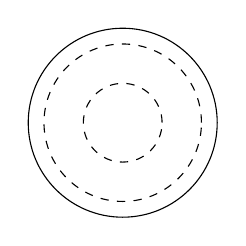
\begin{tikzpicture}
\draw[style=dashed] (0,0) circle (0.5);
\draw[style=dashed] (0,0) circle (1);
\draw(0,0) circle (1.2);
\end{tikzpicture}
\end{tcblisting}


\begin{tcblisting}{listing side text,righthand width=2.5cm}
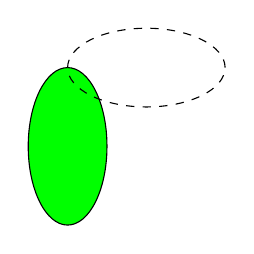
\begin{tikzpicture}
\draw[fill=green] (1,1) ellipse (.5 and 1); %长短轴
\draw[style=dashed] (2,2) ellipse (1 and .5);
\end{tikzpicture}
\end{tcblisting}

\begin{tcblisting}{listing side text,righthand width=2.5cm}
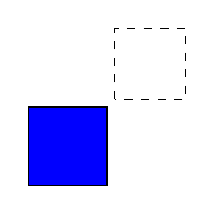
\begin{tikzpicture}
\draw[fill=blue] (0,0) rectangle (1,1);
\draw[style=dashed] (1.1,1.1) rectangle (2,2);
\end{tikzpicture}
\end{tcblisting}


\begin{tcblisting}{listing side text,righthand width=3cm}
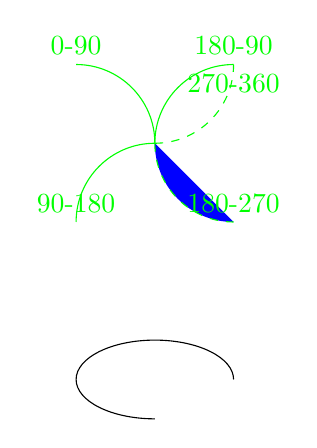
\begin{tikzpicture}
\draw[green] (-1,0) arc(0:90:1)node[above]{0-90};
\draw[green] (-1,0) arc(90:180:1)node[above]{90-180};
\draw[green] (-1,0) arc(180:90:1)node[above]{180-90};
\draw[style=dashed,green,fill=blue] (-1,0) arc(180:270:1)node[above]{180-270};
\draw[green,style=dashed] (-1,0) arc(270:360:1)node[below]{270-360};

\draw (0,-3) arc (0:270: 1 and 0.5);
\end{tikzpicture}
\end{tcblisting}


\begin{tcblisting}{listing and text}
\begin{tikzpicture}
\draw[blue] (0, 0.5)
     .. controls ++ (165:-1) and ++ (240: 1) .. ( 3, 2)
     .. controls ++ (240:-1) and ++ (165:-1) .. ( 2, 4)
     .. controls ++( 165:1)  and ++ (175:-2) .. (-1, 2)
     .. controls ++(175: 2) and  ++ (165: 1) .. ( 0,.5);
\draw( -3.5,1) parabola bend ( -2.5,0)(1.414 ,2);
\draw[green] ( -2,-2) .. controls ( -1,0) .. ( 1,-1);
\draw[red] (0, -3) .. controls (1,-2) and (1.5,-3).. (2,-3);
\end{tikzpicture}
\end{tcblisting}
\subsection{坐标系}

\begin{tcblisting}{listing and text}  
\begin{tikzpicture}[scale=0.8]
\draw[->] (-5.2,0)--(5.2,0);
\draw[->] (0,-5.2)--(0,5.2);      %xy轴坐标

\foreach \x in {0,1,...,8}
{
	\draw[xshift=\x cm] (-4,0) -- (-4,0.1);
	\draw[yshift=\x cm] (0,-4) -- (0.1,-4);
};                               %刻度

\node[below] at (0.2,0){0};      %坐标原点

\foreach \x in {-4,-3,...,-1}
\node[below] at(\x,0){\x};
\foreach \y in {1,2,...,4}
\node[below] at(\y,0){\y};      %x轴刻度

\foreach \y in {-4,-3,...,-1}
\node[left] at(0,\y){\y};
\foreach \y in {1,2,...,4}
\node[left] at(0,\y){\y};     % y轴刻度
\end{tikzpicture}
\end{tcblisting}

\subsection{函数图像}
\myverb{\usepackage{pgfplots}}

\begin{tcblisting}{listing and text,title={$ \operatorname{sigmoid}(\mathbf{x})=\frac{1}{1+e^{-x}} $}}  
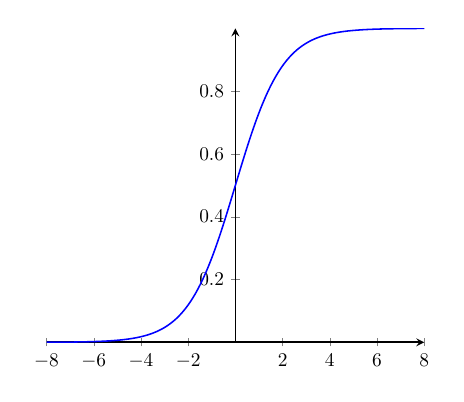
\begin{tikzpicture}[scale = 0.7]  
    \begin{axis}[axis lines=middle,  %坐标轴属性设置
       samples=200,      %切分格大小            
       thick,
       domain=-8:8,      %函数范围
       legend pos=outer north east,
       smooth]
       \addplot+[no marks]{{1/(1+(e^(-1*(\x))))}};    
     \end{axis}
\end{tikzpicture}
\end{tcblisting}

\begin{tcblisting}{listing and text,title={$ \operatorname{ReLU}(\mathbf{x})=\max (\mathbf{x}, 0) $}}  
\begin{tikzpicture}[scale = 0.7] 
\begin{axis}[
axis lines=middle,
samples=200,
%    grid,
thick,
domain=-8:8,
legend pos=outer north east,
smooth,
]
\addplot+[no marks]{max(\x,0)};
\end{axis}
\end{tikzpicture}
\end{tcblisting}

\begin{tcblisting}{listing and text,title={ $ \tanh (\mathbf{x})=\frac{e^{\mathbf{x}}-e^{-\mathbf{x}}}{e^{\mathbf{x}}+e^{-\mathbf{x}}} $ }}  
\begin{tikzpicture}[scale = 0.7] 
\begin{axis}[
axis lines=middle,
samples=200,
%    grid
thick,
domain=-8:8,
legend pos=outer north east,
smooth,
]
\addplot+[no marks]{((e^(1*(\x)))-(e^(-1*(\x))))/((e^(1*(\x)))+(e^(-1*(\x))))};
\end{axis}
\end{tikzpicture}
\end{tcblisting}


\begin{tcblisting}{listing and text,title={ $ \operatorname{SELU}(\mathbf{x})=\lambda\left\{\begin{array}{ll}
				\mathbf{x}, & \text { if } \mathbf{x}>0 \\
				\alpha e^{\mathbf{x}}-\alpha, & \text { if } \mathbf{x} \leq 0
			\end{array}\right. $ }}  
\begin{tikzpicture}[scale = 0.7] 
\begin{axis}[
axis lines=middle,
samples=200,
%    grid,
thick,
domain=-8:8,
legend pos=outer north east,
smooth,
]
\addplot[domain=-8:0,blue,thick,]         % 设置函数的定义域
{1*(e^(1*(\x)))-1};                       % 输入显式函数
\addplot[domain=0:8,blue,thick,]          % 设置函数的定义域
{x};                                      % 输入显式函数 
\end{axis}
\end{tikzpicture}
\end{tcblisting}
嘻嘻
\begin{tcblisting}{listing and text,title={ $ \operatorname{softmax}\left(\mathbf{x}_{i}\right)=\frac{e^{\mathbf{x}_{i}}}{\sum_{j=0}^{k} e^{\mathbf{x}_{k}}} $ }}  
\begin{tikzpicture}[scale = 0.7] 
\begin{axis}[
axis lines=middle,
samples=200,
%    grid,
thick,
domain=-8:8,
legend pos=outer north east,
smooth,
]
\addplot+[no marks]{((e^(0.1*(\x)))-(e^(-1*(\x))))/((e^(0.1*(\x)))+(e^(-1*(\x))))};
\end{axis}
\end{tikzpicture}
\end{tcblisting}

\begin{tcblisting}{listing and text}  
	
\end{tcblisting}





\section{一些例子}
\begin{tcblisting}{listing and text}  
\begin{tikzpicture}[>=latex,scale=1]
\node (k1) at (2,0)[rectangle,draw=black,fill=white]{控制器};
\node (k2) at (6,0)[rectangle,draw=black,fill=white]{被控对象};

\draw[->](-1,0)--node[above]{输入量}node[below]{$ r(t) $}(k1);
\draw[->](k1)--node[above]{控制作用}node[below]{$ u(t) $}(k2);
\draw[->](k2)--node[above]{输出量}node[below]{$ y(t) $}(9,0);
\end{tikzpicture}
\end{tcblisting}


\begin{tcblisting}{listing and text}  
\begin{tikzpicture}[>=latex,scale=1]
\node (k1) at (2,0)[rectangle,draw=black,fill=white]{计算(电位器) };
\node (k2) at (6,0)[rectangle,draw=black,fill=white]{执行(功率放大器)};
\node (k3) at (10,0)[rectangle,draw=black,fill=white]{对象(电动机)};

\draw[->](-1.5,0)--node[above]{输入量}(k1);
\draw[->](k1)--(k2);
\draw[->](k2)--(k3);
\draw[->](k3)--node[above]{输出量}(13.5,0);
\draw[->](10,1.2)--node[right]{扰动}(k3);
\end{tikzpicture}


\end{tcblisting}


\begin{tcblisting}{listing and text}  
\begin{tikzpicture}[>=latex,scale=1]
\node (k1) at (2.5,0)[rectangle,draw=black,fill=white]{控制器 };
\node (k2) at (6,0)[rectangle,draw=black,fill=white]{控制对象};
\node (k3) at (4.5,-2)[rectangle,draw=black,fill=white]{反馈元件};
\node at (-.4,.2)[rectangle,draw=white,fill=white]{+};
\node at (-.2,-.4)[rectangle,draw=white,fill=white]{-};

\draw (0,0) circle (0.2);
\draw (-.1414,.1414)--(.1414,-.1414);
\draw (.1414,.1414)--(-.1414,-.1414);

\draw[->](-2.5,0)--node[above]{输入量}(-.2,0);
\draw[->] (0.2,0)--node[above]{误差}(k1);
\draw[->] (k1)--node[above]{控制量}(k2);
\draw[->] (k2)--node[above]{输出量}(9.5,0);
\draw[->] (9,0)--(9,-2)--(k3);
\draw[->] (k3)--(0,-2)--(0,-0.2);
\end{tikzpicture}
\end{tcblisting}
\myverb{\usepackage[european]{circuitikz}}

\begin{tcblisting}{listing and text}  
\begin{tikzpicture}[>=latex,scale=1]
\node (k1) at (3,0)[rectangle,draw=black,fill=white]{控制单元};
\node (k2) at (7.5,0)[rectangle,draw=black,fill=white]{控制对象};
\node (k3) at (4.5,-2)[rectangle,draw=black,fill=white]{反馈元件};
%\node at (-.4,.2)[rectangle,draw=white,fill=white]{+};
\node at (-.2,-.4)[rectangle,draw=white,fill=white]{-};
\node at (3,-.7)[rectangle,draw=white,fill=white]{$ G_{1} $};
\node at (7.5,-.7)[rectangle,draw=white,fill=white]{$ G_{2} $};
\node at (4.5,-2.7)[rectangle,draw=white,fill=white]{$ H $};

\draw (0,0) circle (0.2);
\draw (-.1414,.1414)--(.1414,-.1414);
\draw (.1414,.1414)--(-.1414,-.1414);

\draw[->](-3,0)--node[above]{给定信号$r(t)$}(-.2,0);
\draw[->] (0.2,0)--node[above]{误差$e(t)$}(k1);
\draw[->] (k1)--node[above]{控制量$u(t)$}(k2);
\draw[->] (k2)--node[above]{输出$y(t)$}(11,0);
\draw[->](7.5,1.4)--node[right]{扰动$n(t)$}(k2);
\draw[->] (9,0)--(9,-2)--(k3);
\draw[->] (k3)--(0,-2)--node[right]{主反馈$b(t)$}(0,-0.2);
\end{tikzpicture}
\end{tcblisting}




\begin{tcblisting}{listing and text}  
\begin{circuitikz}
    \draw (.5,0) to[short, o-, i=$i$](1.5,0)
    to [R=$R$] (3,0)
    to[short, -o] (5,0)
    (3.5,0) to[C=aaa, l_=$C$, *-*](3.5,-2)
    to[short, -o] (.5,-2)
    (3.5,-2) to[short, -o](5,-2);

    \node at (0.5,-1)[rectangle,draw=white,fill=white]{$ u_{i} $};
    \node at (5,-1)[rectangle,draw=white,fill=white]{$ u_{o} $};
\end{circuitikz}
\end{tcblisting}



\begin{tcblisting}{listing and text}  
\begin{circuitikz}
\draw (.5,0) to[short, o-, i>^=$i_1$](1.5,0)
to [R=$R_1$] (3,0)--(3.8,0)
to [R=$R_2$](6,0)
(6,0) to[short, -o] (7.5,0)
(3.5,0) to[C, l=$C_{1}$, *-*](3.5,-2)
to[short, -o] (.5,-2)
(6,-2) to[short, -o](7.5,-2)
(6,0) to[C, l=$C_{2}$, *-*,i>^=$i_2$](6,-2)
(6,-2)--(3.5,-2)
{[anchor=south] (3.5,0) node {$ u_{1} $}} ;

\node at (0.5,-1)[rectangle,draw=white,fill=white]{$ u_{i} $};
\node at (7.5,-1)[rectangle,draw=white,fill=white]{$ u_{o} $};		
\end{circuitikz}
\end{tcblisting}



\begin{tcblisting}{listing and text}  
\begin{circuitikz}[scale=0.8,>=latex]
\draw(3.5,-.5) node [op amp] (opamp) {}
(-1.5,.1) node [below] {$u_{i}(t)$} to [R, l=$R_3$, o-*,i>^=$i_{1}(t)$] (2,.1)
to  (opamp.-)|-(2.5,2) 
to [R, l=$R_{1}$] (4,2)
to [C, l=$C_{1}$, -*](6,2)
to [C, l=$C_{2}$](6,0.3) to node[rground]{}(6,1)
(6,2) to[R, l=$R_{2}$] (8.5,2) to[short,i>^=$i_{2}(t)$](8.5,-.5) 

(opamp.+) to [R, l_=$R_{4}$, *-](2,-3)
to node[rground]{}(2,-2.9)
(opamp.out) to [short,-*] (8.5,-.5) 
to [short, -o](9.5,-.5) node [below] {$u_{c}(t)$}
{[anchor=south] (6,2) node {$ u_{1}(t) $} };
\draw[->] (2,.1) -- (1.5,-0.5)node[left]{A};
\draw[->] (6,2) -- (5,1)node[left]{C};
\end{circuitikz}
\end{tcblisting}

\section{3D}
\begin{tcblisting}{listing and text}  
\begin{tikzpicture}[z={(10:10mm)},x={(-45:5mm)}]
\def\wave{
\draw[fill,thick,fill opacity=.2]
(0,0) sin (1,1) cos (2,0) sin (3,-1) cos (4,0)
sin (5,1) cos (6,0) sin (7,-1) cos (8,0)
sin (9,1) cos (10,0)sin (11,-1)cos (12,0);
\foreach \shift in {0,4,8}
{
\begin{scope}[xshift=\shift cm,thin]
\draw (.5,0) -- (0.5,0 |- 45:1cm);
\draw (1,0) -- (1,1);
\draw (1.5,0) -- (1.5,0 |- 45:1cm);
\draw (2.5,0) -- (2.5,0 |- -45:1cm);
\draw (3,0) -- (3,-1);
\draw (3.5,0) -- (3.5,0 |- -45:1cm);
\end{scope}
}
}
\begin{scope}[canvas is zy plane at x=0,fill=blue]
\wave
%\node at (6,-1.5) [transform shape] {magnetic field};
\end{scope}
\begin{scope}[canvas is zx plane at y=0,fill=red]
\draw[help lines] (0,-2) grid (12,2);
\wave
%\node at (6,1.5) [rotate=180,xscale=-1,transform shape] {electric field};
\end{scope}
\end{tikzpicture}
\end{tcblisting}


\begin{tcblisting}{listing and text}  

\end{tcblisting}

\begin{tcblisting}{listing and text}  

\end{tcblisting}

\end{document}

